\section{Keypad}
To take user input a keypad with 12 keys is used, see \cref{fig:keypad}. \cite{rspro} 
This was chosen to have a simple user interface for the user to input numbers and has been extended to handle input as letters also.
There is a long delay after the button has been released until the output is changed. 
This means there is added a delay in different parts of the code to make sure enough time has passed for the keypad to change. 
Another possibility would be using the touch screen of the graphic display. 
It could have been implemented with a variable amount of keys shown on the display. 
This would reduce the number of components since the touchscreen is already a part of the display. 
The downside of using the screen for user input is that it takes up space on the display. This means there is less space for showing relevant information for the user.

\begin{figure}[H]
\centering
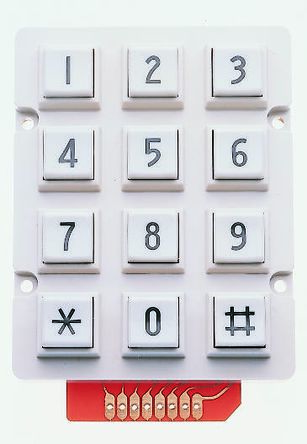
\includegraphics[width=0.3\linewidth]{graphics/keypad}
\caption{The keypad is the user interface to get input from the user. Square button is used as enter and star button is used to delete input.}
\label{fig:keypad}
\end{figure}


\subsection{Keypad Scan}
The keypad has its keys placed in a $4\times3$ matrix layout. 
There are 8 pins with 4 rows, 3 columns and 1 SC pin connected to ground. 
The 3 column pins are set high one at a time by bit shifting through \mintinline{c}{PORTL} bit \mintinline{c}{2, 1, 0}. 
The 4 row pins are pulled to ground with pull down resistors.
When a key is pressed a connection between a column, which is high, and a row which is low will happen.
This will set the row high. 
The 4 row pins are set as inputs, with one row checked at a time by bit shifting through \mintinline{c}{PINL} bit \mintinline{c}{7, 6, 5, 4}. \cite{matrixkeypad}
The \mintinline{c}{NumKeyScan} function returns a number between 1-12, with 1 = 1, 2 = 2, ..., \# = 12. 

\subsection{Keypad Numbers}
To use the keypad for numbers only, the input from the keypad scan is added with 48 turning the input to the corresponding ASCII numbers. The numbers are shown on the display with a large font as each number is entered. The number is then stored in a char array which is used when the user has finished entering numbers. To delete numbers the star key has been chosen. This deletes the number from the display and from the char array.

\subsection{Keypad Letters}
To use the keypad to enter letters or numbers, it is used as an telephone keypad according to the international standard. \cite{keypad} This means the number 2 also represents a, b and c. Every key has a struct containing the different possible characters. It also contains the amount of characters and the current position. 
A timer is implemented using an interrupt. If there has been a keypad input with the same value as before and the timer is lower than the threshold, the position is moved. The corresponding letter is then shown on the display. If a new key is pressed the timer is reset. The threshold is set at \SI{2}{\second} to make sure the user has time to input a new character. The keypad is quite slow mechanically so a longer delay is required. The characters selected by the user is shown on the display as text when the user presses a key. If it is pressed before the timer runs out the old character is overwritten with a new character. The star key has been chosen to delete characters if pressed. The name is stored in a char array until the user is finished inputting the letters.
